\begin{post}
	\postdata{Strikeout}{2011}{10}{2}{22}{5}{6}
	\begin{content}
The last time I have been to a baseball match was two years ago, when Kotlářka played at Markéta. And that was only as a spectator. I don't even remember the exact date of my last game as a player --- I only remember it was the final game of the 2004 Czech championship, where we played against Krč, and despite our underdog position, we managed to keep up until around 7th inning. We lost, unfortunately, but for me the silver medal was nearly as valuable as the gold one from the previous year, because we had a ``weaker'' team. Hmm, I think I got carried away a little.

Anyway, me and other intl students from KAIST decided to go see baseball game at the Jamsil Stadium. You might not know that, but baseball is one of the most favorite sports here. The professional league comprises 8 teams, and since now it's getting into its post-season phase, it is one of the hottest topics among sports fans in Korea.

We went to see a derby between Doosan Bears and LG Twins. The teams in KBO league are named after a sponsor instead of a city, and they sometimes take inspiration from the MLB (Twins, Lotte Giants, Kia Tigers). This two teams don't stand a chance getting into the post-season, so it was merely a game of honor for them, because both come from Itaewon and both have the Jamsil Stadium as their home ball park. Because the Bears part of the stadium was already sold out long before the game, we had to get seats in Twins' section. As it turned out later, that was the only glitch of the game.

\begin{wrapfigure}[12]{R}{0.46\textwidth}
\centering
\fbox{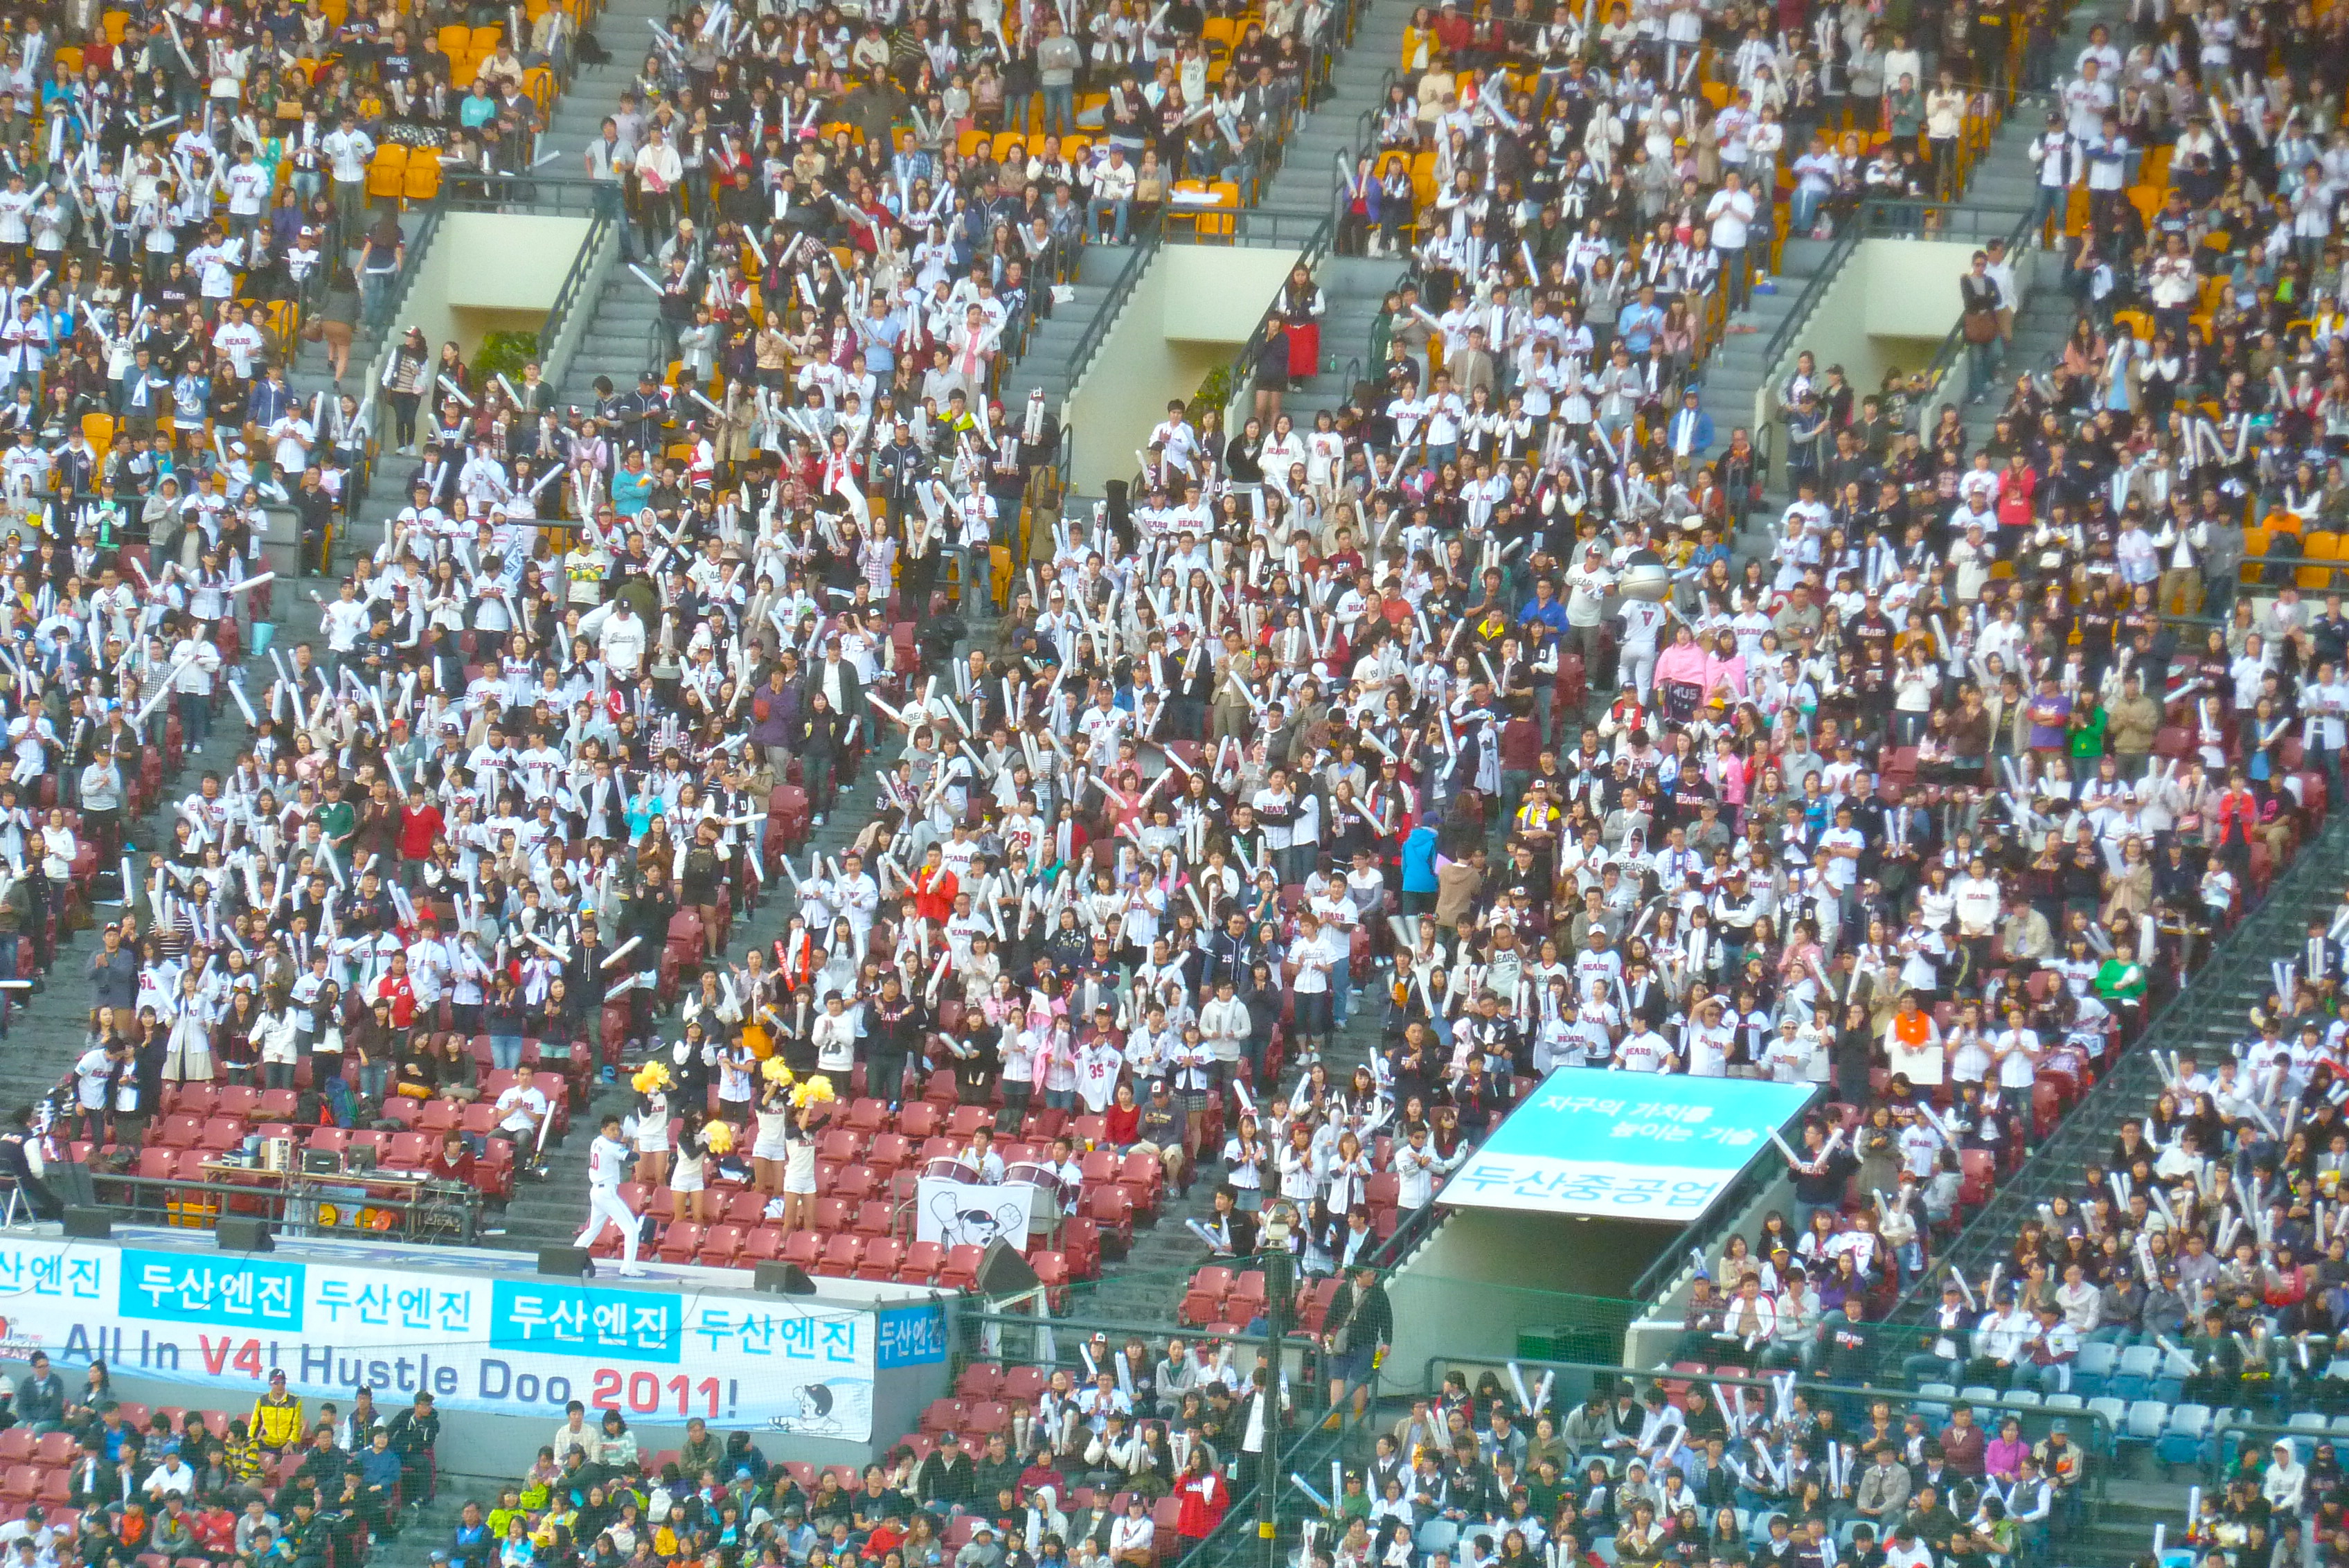
\includegraphics[width=0.46\textwidth]{photos/10/02/cheering-sticks.jpg}}
\caption{Doosan fans with white cheering sticks}
\vspace{-24pt}
\end{wrapfigure}

Baseball in Korea is not only a sport, but also a show. People come to watch the game and have a tremendous amount of fun. Each team has own cheerleaders and an entertainer that tells people what to do. Since everybody has a cheering stick, the stands turn into a sea of red/white/\ldots every time people go crazy. It's impressive. Moreover, (almost) every player has it's own song that is played through the PA when he's at bat, and of course, all the people know these songs, so with every new player the stadium (or at least half of it) turns into a huge karaoke. Every good action leads to another wave of craziness, even if it's just a single hit. You can't even imagine what happens when someone scores a homerun.

As I said, our location was not perfect. From unknown reasons the Twins fans are not as crazy as the ones of Bears, so our side of the stadium was rather lame. This was also caused by the development of the game, because even though the teams were tied in second, from fourth on Bears started kicking Twins' ass. The main reason were the Twins' pitchers, giving BBs and serving nice hitting material to Doosan hitters. I was quite surprised by the eventual humiliation (9:1), because Bears are the second to last team while Twins are 5th, the first team not to go to the play-offs. Despite the loss, I have really enjoyed the match. Watching nice baseball after so may years really brought back my baseball memories and reminded me of all the nice moments of my career.

\begin{figure}[h]
\centering
\subfigure[The stadium]{\fbox{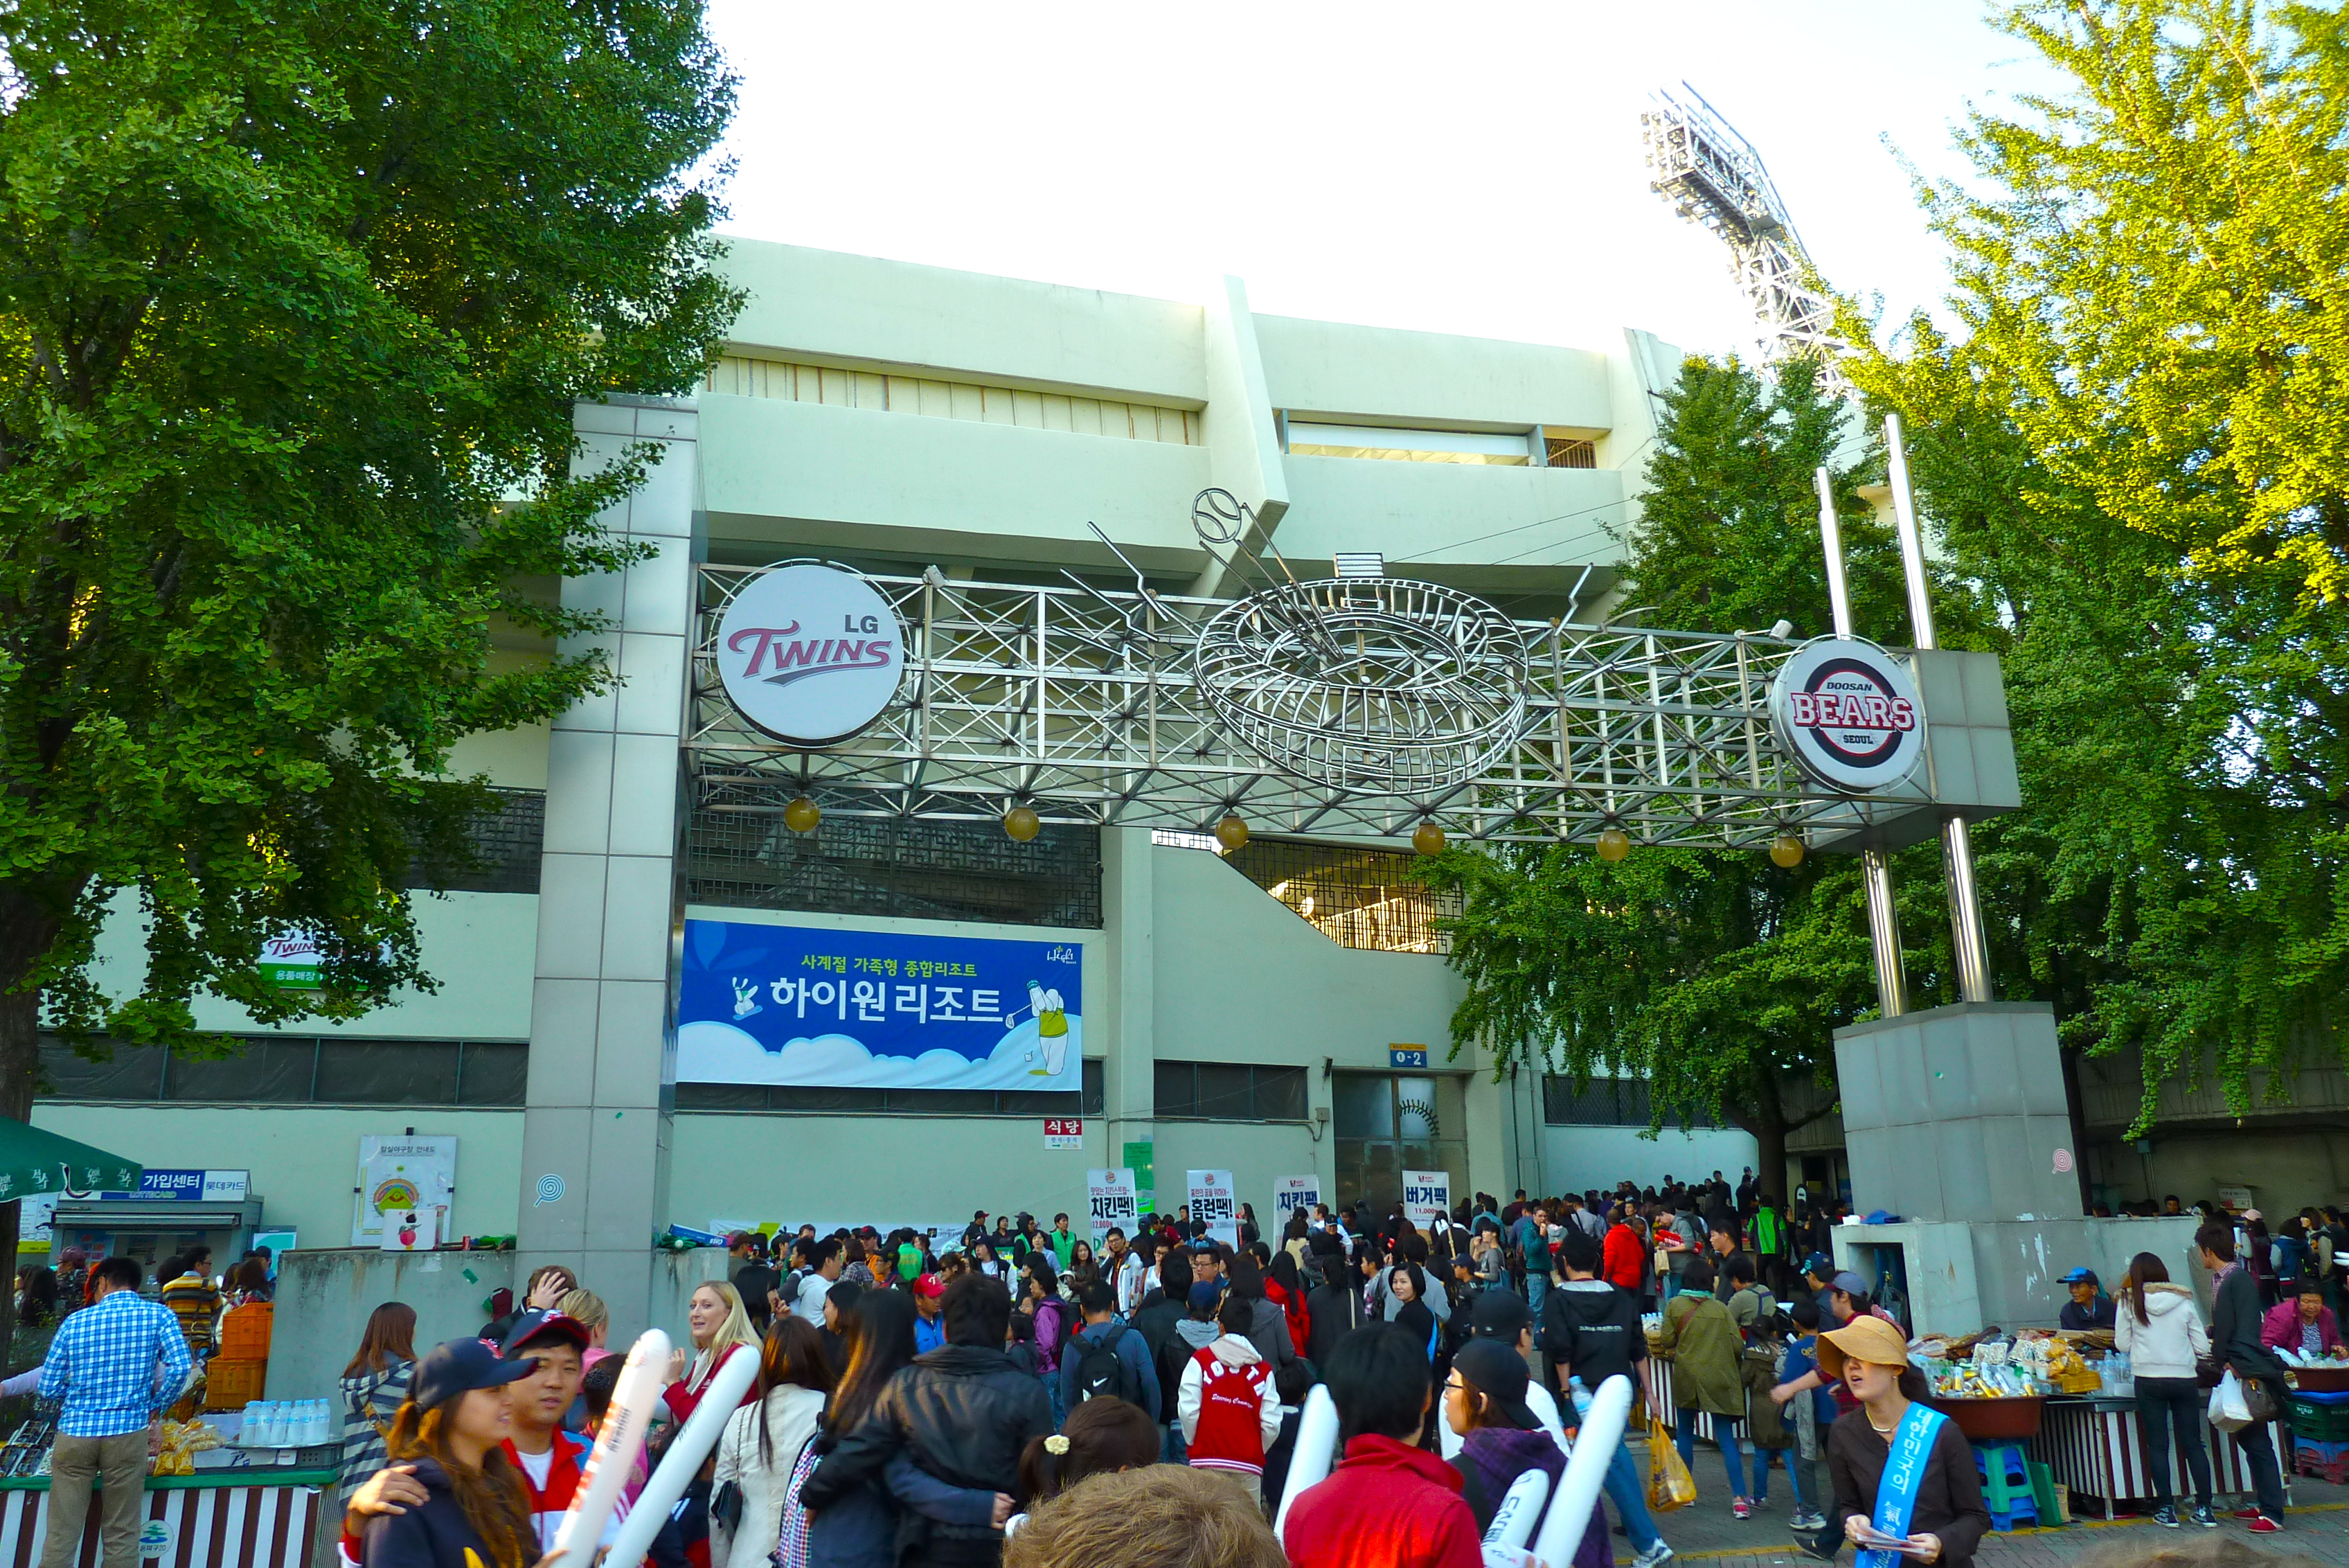
\includegraphics[width=0.45\textwidth]{photos/10/02/P1000569.jpg}}}
\subfigure[Beautiful sunset]{\fbox{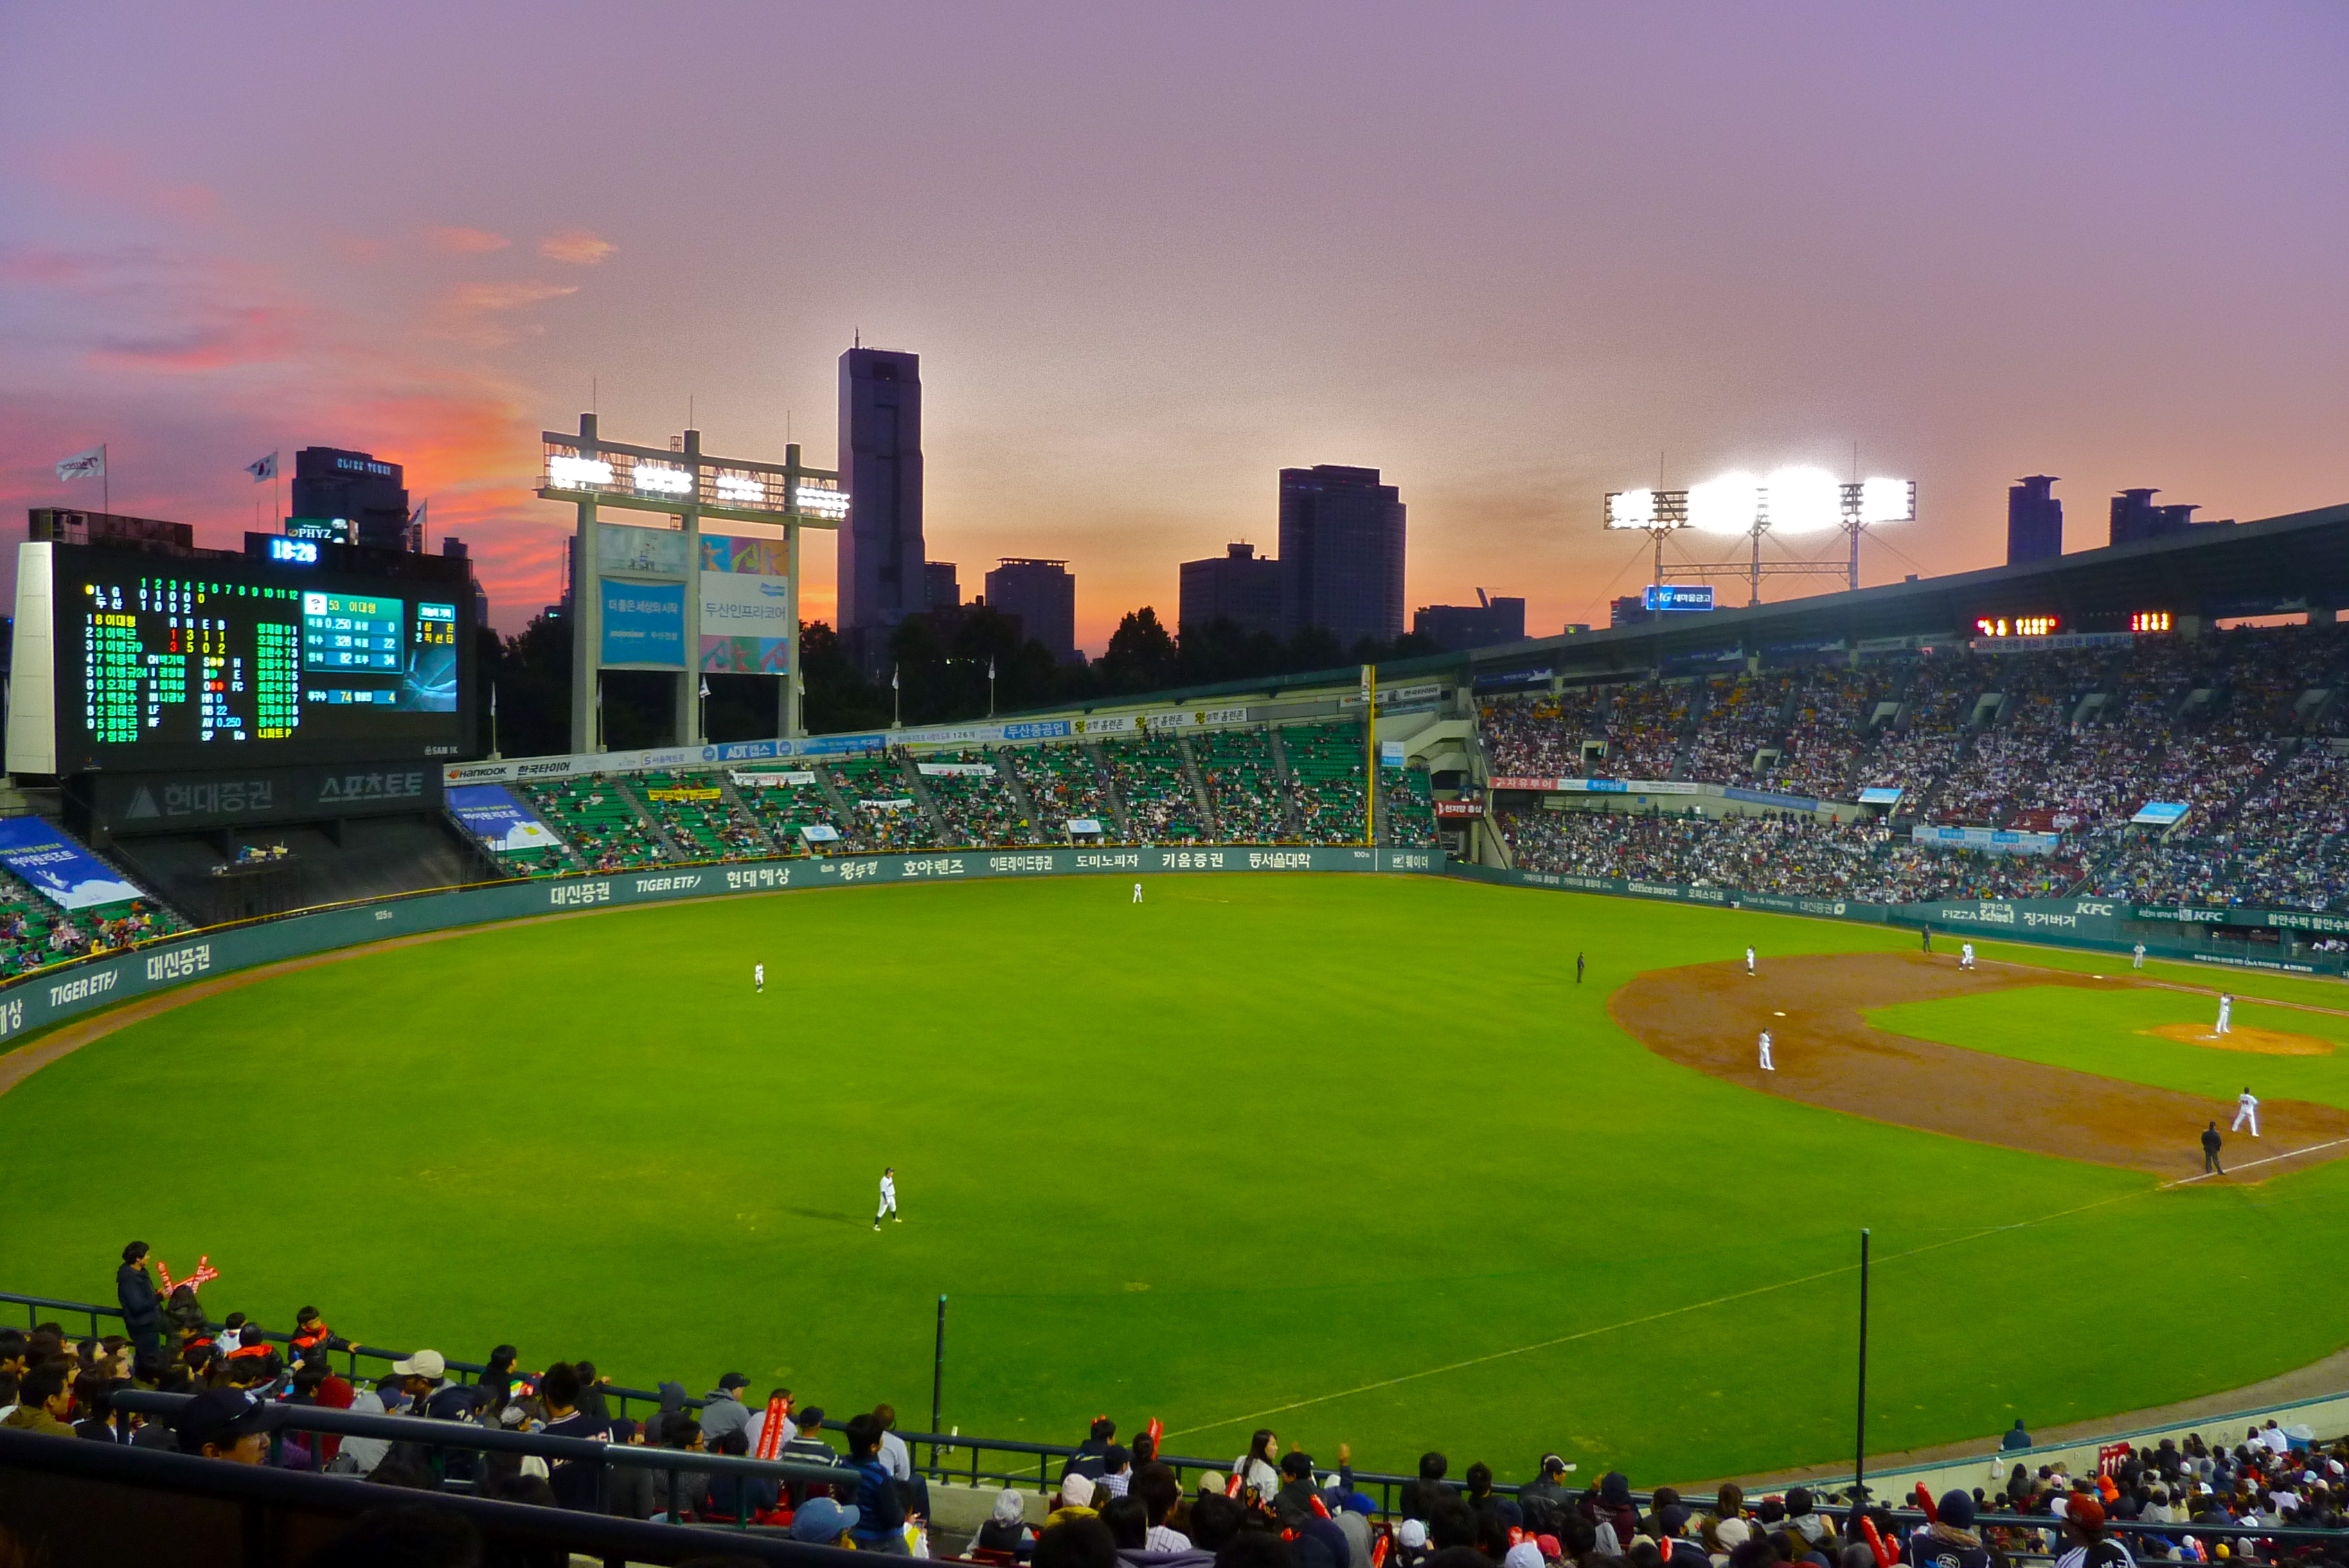
\includegraphics[width=0.45\textwidth]{photos/10/02/P1000598.jpg}}}
\subfigure[The game is on]{\fbox{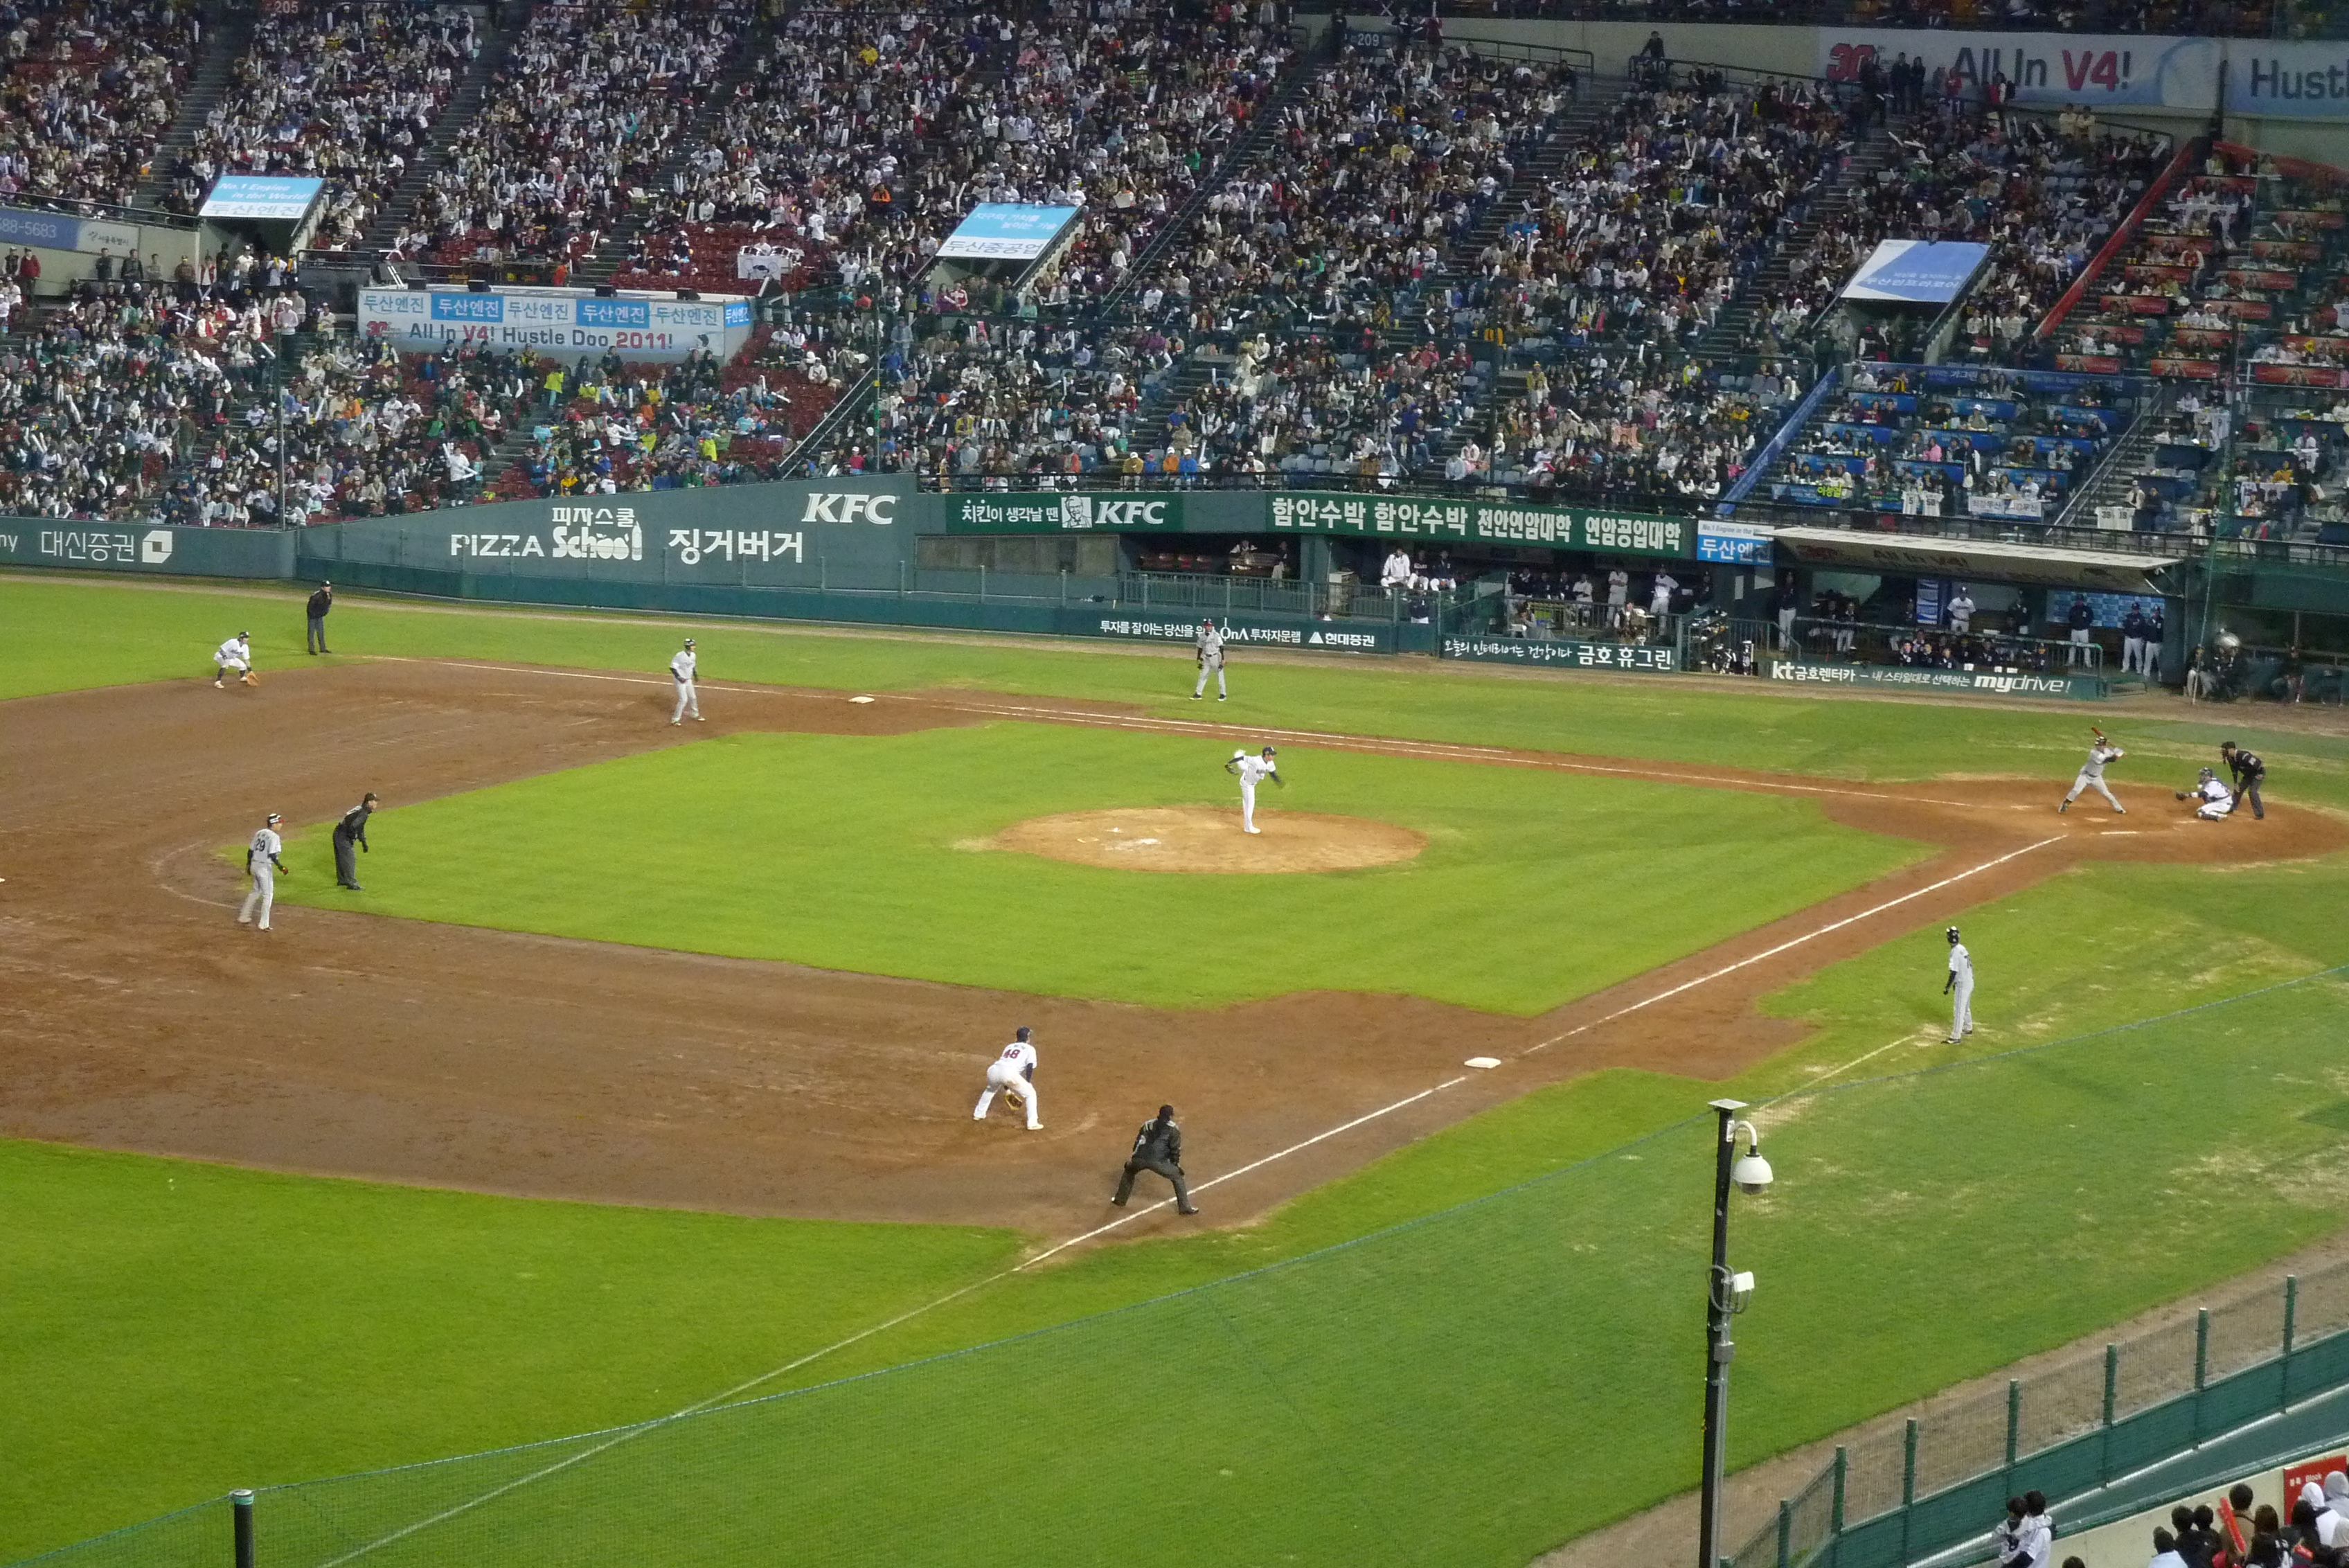
\includegraphics[width=0.45\textwidth]{photos/10/02/P1000641.jpg}}}
\subfigure[``Our'' cheerleaders]{\fbox{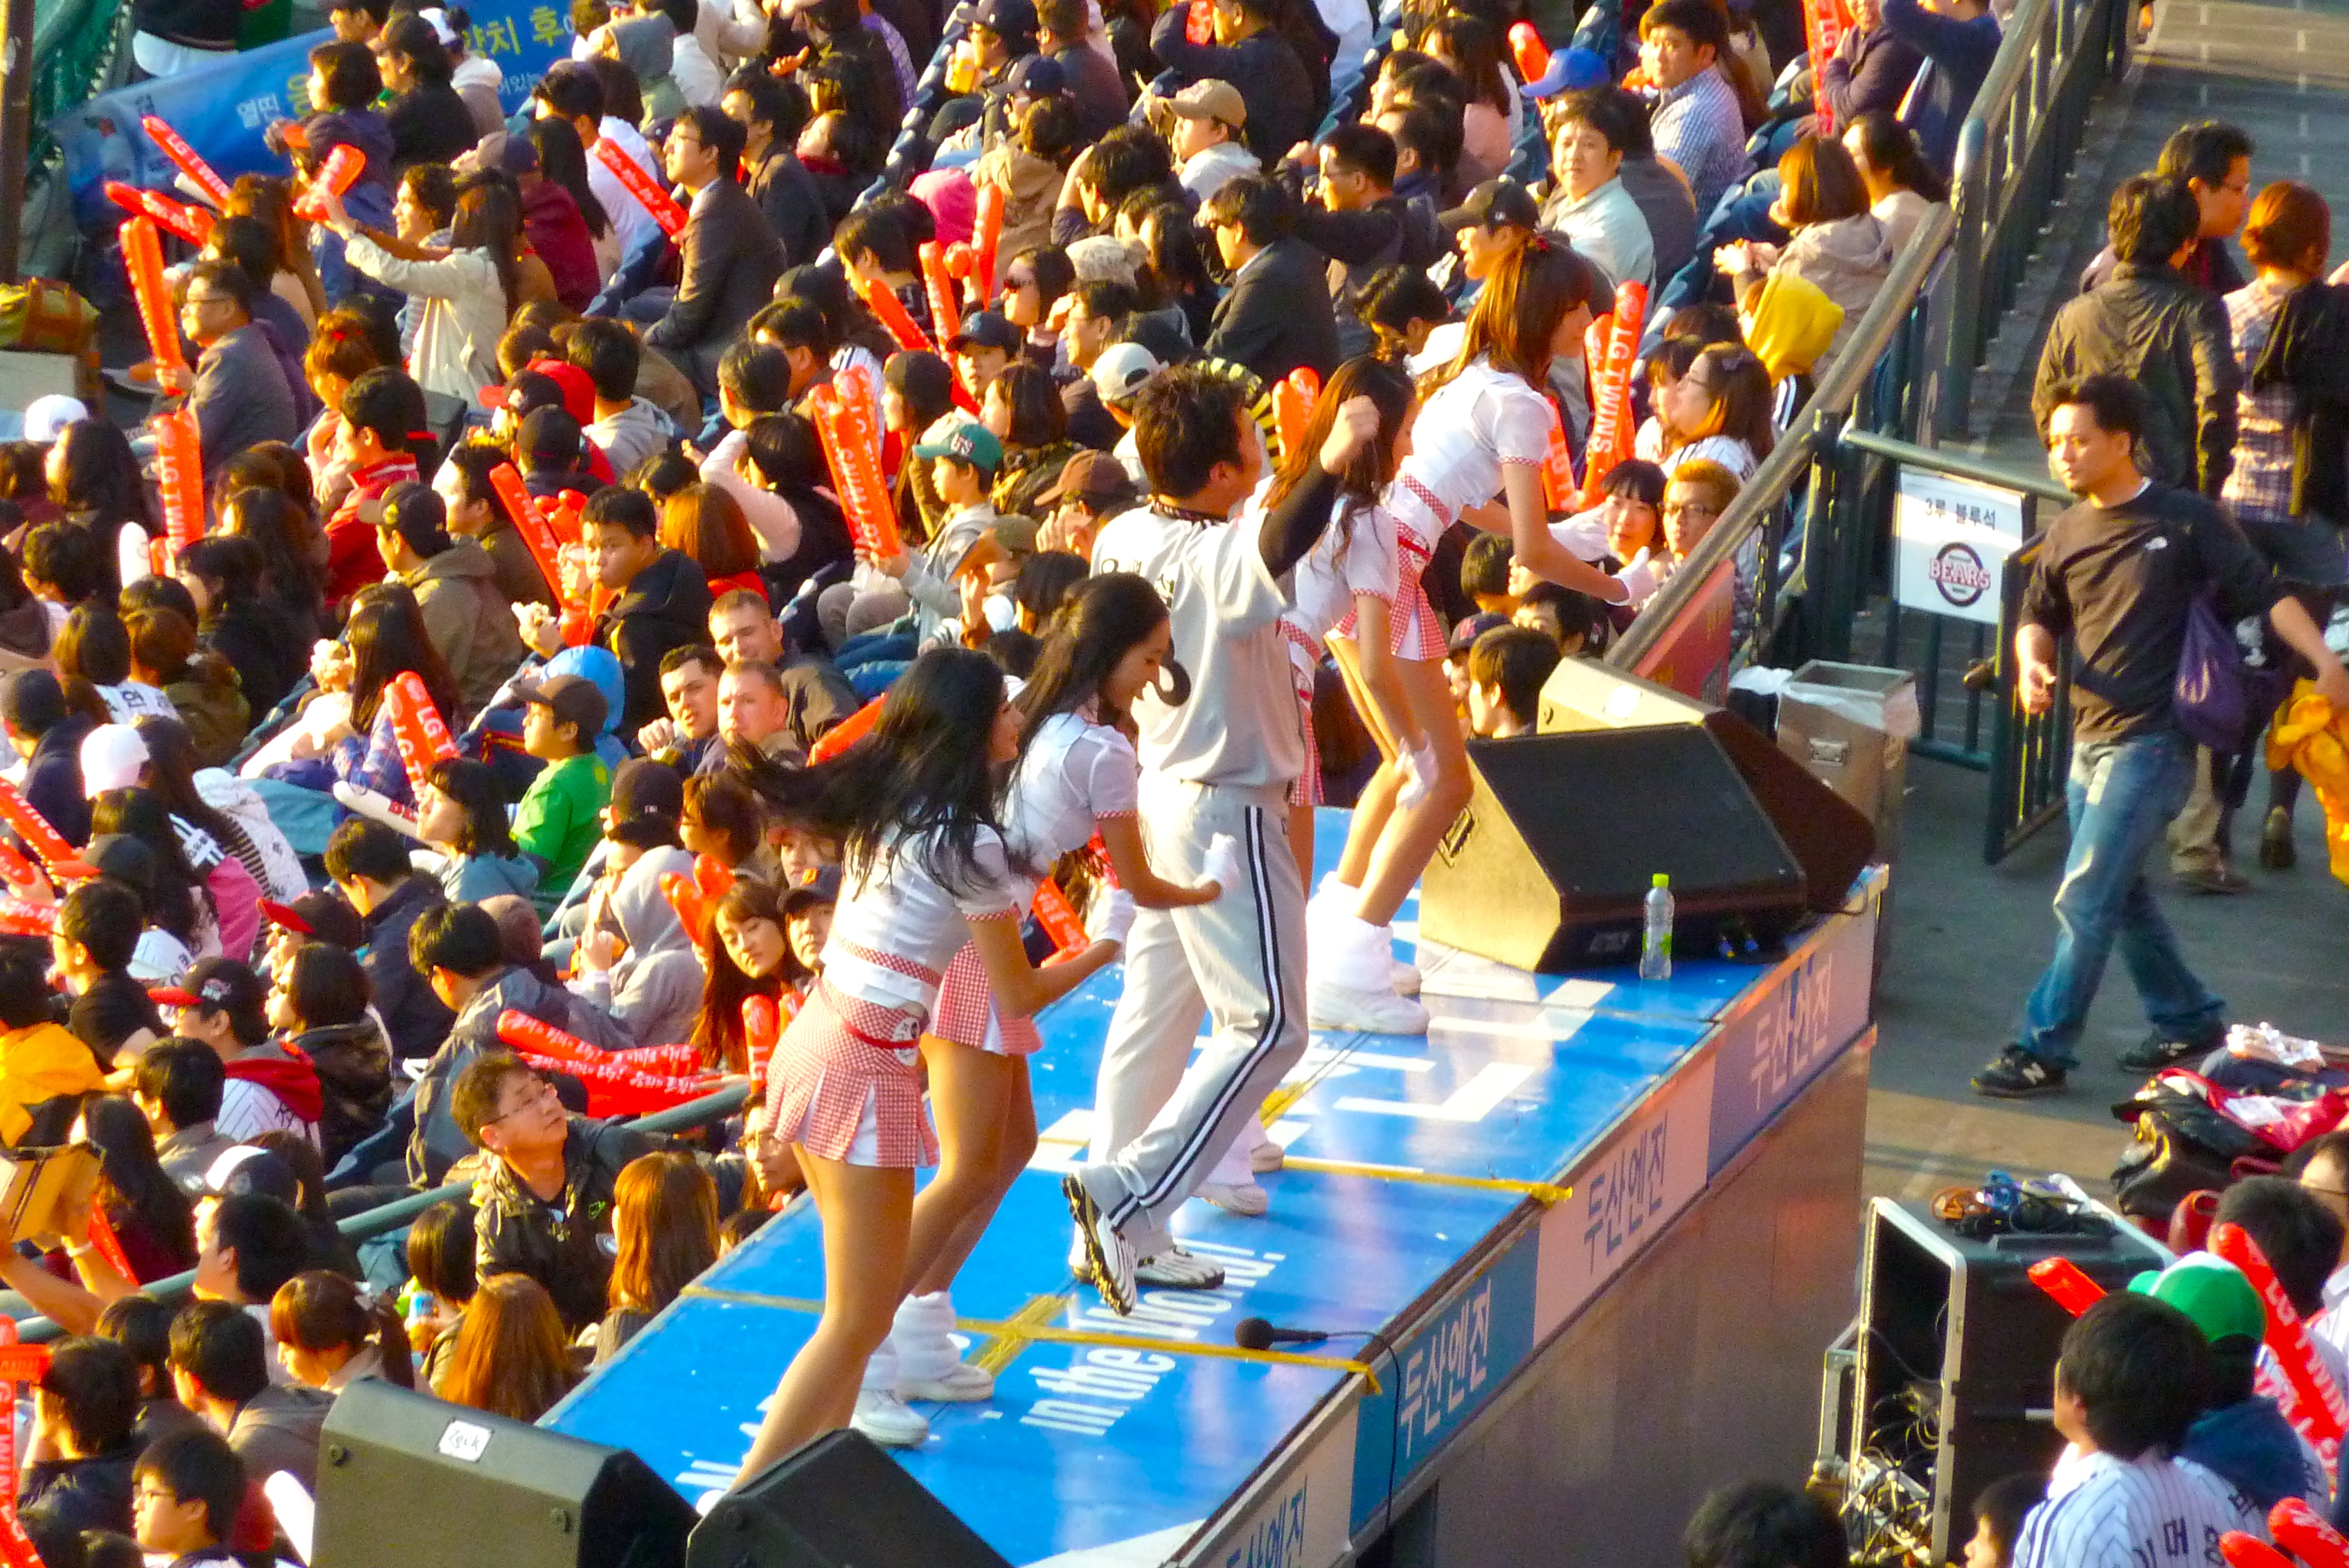
\includegraphics[width=0.45\textwidth]{photos/10/02/P1000584.jpg}}}
\end{figure}


%Here are some pictures I took that day. In the morning I was in Gangnam, where I had a meeting with my Delft classmate Ferdian about one project so some photos are from there.


	\end{content}
\end{post}
